\chapter{Tor wizyjny}
\label{cha:torwizyjny}

Kolejnym krokiem realizacji projektu była implementacja podstawowych zadań przetwarzania obrazu w logice rekonfigurowalnej układu heterogenicznego. 
Rozpoczęto od stworzenia podstawowego toru wizyjnego pobierającego obraz z wejścia HDMI i~wysyłającego go bez zmian na wyjście VGA. 
Następnie stworzono moduły pozwalające na realizację algorytmu śledzenia przez detekcję.

\section{Podstawowe przesyłanie obrazu}
\label{sec:podstawoweprzesylanieobrazu}
Tor wizyjny nie wykonujący żadnych zmian w obrazie pozwoli nam na określenie czy dane są poprawnie odbierane z kamery i poprawnie wysyłane do monitora. 
Stanowić on będzie również bazę dla dowolnego innego realizowanego algorytmu przetwarzania obrazu. 
Konieczna jest więc pewność, że działa poprawnie. 
Musi on realizować następujące zadania:
\begin{enumerate}
\item Odbieranie danych ze złącza HDMI/DVI.
\item Dekodowanie danych odebranych ze złącza HDMI/DVI do postaci przestrzeni barw RGB i sygnałów synchronizacyjnych.
%TODO nie podoba mi się to stwierdzenie. one po HDMI są przesyłane w RGB więc to nie ma konwersji. Jest dekodowanie do postaci RGB i sychronizacji -zrobione.
\item Kodowanie danych z przestrzeni barw RGB i sygnałów synchronizacyjnych do VGA.
%TODO jw. -zrobione.
\item Wysłanie danych do złącza VGA.
\end{enumerate}
Zadania te są realizowane przez moduły dostarczane przez firmę \textit{Digilent}, producenta platformy obliczeniowej.
Moduły połączone zostały w schemacie blokowym programu \textit{Vivado}, co pokazano na rysunku \ref{fig:tor_wizyjny}.
%TODO co to znaczy, że za pomocą diagramu ??? styl -zrobione.
Schemat blokowy, w porównaniu do pliku języka Verilog, zwiększa przejrzystość połączeń między modułami oraz zmniejsza ryzyko błędu np. w nazwie portu.
%TODO Odniesienie  w txt do rysunku (do każdego mu być !!!) -zrobione.
%TODO To dla odmiany mogłoby być większe.... na całą szerokość strony. -zrobione.
%TODO Przydałoby się też omówienie posczególych modułów. -zrobione.

\paragraph*{}
Do stworzenia schematu widocznego na rysunku \ref{fig:tor_wizyjny} wykorzystano następujące moduły:\begin{itemize}
\item \textit{Clocking Wizard} - Generacja sygnału zegarowego o częstotliwości \(200\)MHz.
\item \textit{DVI to RGB Video Decoder} - Dekodowanie danych odebranych ze złącza HDMI/DVI do postaci przestrzeni barw RGB i sygnałów synchronizacyjnych.
\item \textit{RGB unpack} - Zamiana 24-elementowego wektora przestrzeni barw do osobnych, 8-elementowych wektorów (R, G, B).
\item \textit{RGB pack} - Zamiana trzech 8-elementowych wektorów (R, G, B) do jednego 24-elementowego wektora przestrzeni barw.
\item \textit{RGB to VGA output} - Kodowanie danych z przestrzeni barw RGB i sygnałów synchronizacyjnych do VGA.
\end{itemize}

\begin{figure}[h]
	\centering
	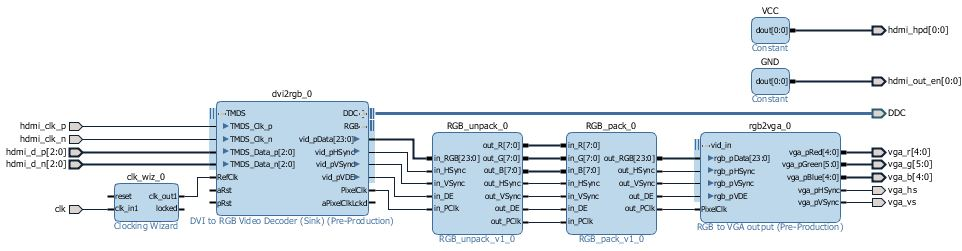
\includegraphics[width=6in]{Tor_wizyjny.jpg}
	\caption{Podstawowy tor wizyjny.}
	\label{fig:tor_wizyjny}
\end{figure}

\paragraph*{}
Testy rozpoczęto od podłączenie wyjścia HDMI laptopa do wejścia HDMI karty ZYBO oraz podłączenia monitora do wyjścia VGA ZYBO. W tak połączonym układzie obraz był wyświetlany poprawnie. Następnie źródło obrazu zamieniono na docelową kamerę. 
W tym przypadku obraz nie został wyświetlony na ekranie monitora. 
W celu znalezienia i naprawy problemu postanowiono w torze wizyjnym włączyć opcję \textit{debug} dla części węzłów. 
Dzięki temu można podglądać sygnały już w działającym układzie.
Ustalono, że problem występuje w module odbierającym dane z wejścia HDMI - \textit{dvi2rgb}. 
Problem udało się naprawić aktualizując go z wersji 1.2 do wersji 1.6, wyłączając bufor dla sygnału zegarowego (opcja \textit{Add BUFG to PixelClk}), włączając opcję \textit{Enable DDC ROM}, zmieniając zakres zegara taktującego TMDS do \(<120\) MHz oraz preferowaną rozdzielczość przetwarzanego obrazu na 1280x720.
%TODO A może Pan napisać szczegóły (do jakich parametrów) -zrobione.

\section{Śledzenie przez detekcję}
\label{sec:sledzenieprzezdetekcje}

Śledzenie przez detekcję zostało zrealizowane na podstawie koloru śledzonego obiektu. 
Jako parametr modułu detekcji podawany jest zakres kolorów w przestrzeni barw RGB, które mają być traktowane jako należące do obiektu. 
Pikselowi, którego kolor mieści się w podanym zakresie przypisywana jest wartość 1, a pozostałym 0. 
Pod nadaniu wartości wszystkim pikselom kadru obliczany jest środek ciężkości obrazu. 
W~ten sposób wyznaczono środek śledzonego obiektu. 
Punkt ten zaznaczany jest na obrazie wyjściowym za pomocą dwóch czerwonych linii - poziomej i pionowej. 
Podczas testów wykrywany był następujący zakres przestrzeni barw RGB, odpowiadający kolorowi zielonemu:
\begin{equation}
R \in [0,30]
\end{equation}
\begin{equation}
G \in [40,255]
\end{equation}
\begin{equation}
B \in [0,30]
\end{equation}
Przykładowy wynik działania opisanego modułu przedstawiono na rysunku \ref{fig:detekcja}.

\begin{figure}[H]
	\centering
	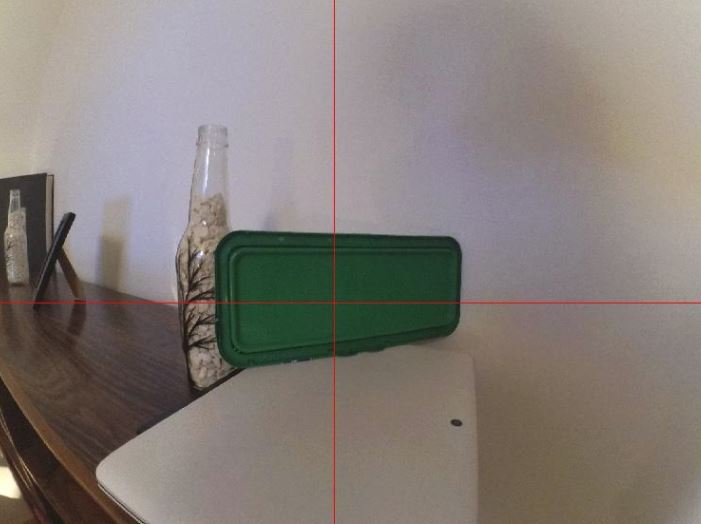
\includegraphics[width=4in]{detekcja.jpg}
	\caption{Przykładowy wynik działania algorytmu.}
	\label{fig:detekcja}
\end{figure}
%TODO odnośnik. No i jakiś mało sugestywny przykład ? to jest w paint ? czy jak ? Nie da się rzeczywistego zdjęcia dać. -zrobiene.

Testy były wykonywane zarówno dla obrazu z komputera PC jak i kamery. 
Należy zwrócić uwagę na niską efektywność tej metody dla obrazu z kamery. 
Spowodowane jest to szumami oraz bardzo dużą zależnością rozpoznanego koloru od natężenia i rodzaju oświetlenia.

\section{Komunikacja PL-PS}
\label{komunikacjapl-ps}

Połączono wykonany w tym rozdziale tor wizyjny i wyznaczanie środka ciężkości z komunikacją zaimplementowaną w rozdziale \ref{cha:komunikacja}.
Dzięki temu zintegrowano stworzone do tej pory moduły w funkcjonalną całość.
W tym celu należało zastosować komunikację pomiędzy procesorem ARM, a FPGA.
%TODO Styl.... trzeba napisać po co - Czy tak lepiej?
Odbywa się ona z użyciem modułu \textit{AXI Lite}.
Do procesora wysyłane są współrzędne wyznaczonego środka ciężkości śledzonego obiektu. 
Kiedy dane są gotowe do odczytu, sygnał oznaczający wysłanie danych do procesora zmienia wartość logiczna z \(0\) na \(1\).
Od narastającego zbocza tego sygnału zgłaszane jest przerwanie, w którym aktualizowana jest zmienna odpowiedzialna za położenie celu, czyli wartości zadane serwomechanizmów. 
W procesorze odebrane współrzędne przeliczone zostają na uchyby regulacji kątów na podstawie rozdzielczości obrazu i kątów nagrywania kamery. 
Założono, że odległość pikseli od środka obrazu jest proporcjonalna do kąta.
Założenie to nie jest słuszne w ogólności, ale jest prawdziwe dla małych wartości odchylenia.
Wyznaczenie dokładnej wielkości wymagałoby użycia Lookup table (tablicy przyporządkowującej każdemu pikselowi wartość kąta) lub wyznaczania funkcji matematycznej wykonującą powyższą funkcję.
%TODO dziwne zdanie...a to nie jest tak, że dla małych kątów...
%MK: Nie wiem czy teraz lepiej. Starałem się to inaczej opisać.
%TODO no ale chyba tylko dla dwóch liczb


%TODO Rozważyłbym jednak śledzenie przez detekcję przenieść przed meanshift, zeby algorytmy śledzące były jeden obok drugiego.
%MK: Pomyślę, co trzebaby wtedy zmienić, żeby to było ok.

%TODO Może jakieś zdjęcie jak to działa, a to było już z serwami robione?
%MK: Kiedy to robiłem to jeszcze nie z serwami, ale później testowałem to z nimi i działało. Ciężko na zdjęciu pokazać, jak się poruszają serwa za obiektem. A samo zdjęcie ze środka ciężkości już jest wyżej. Czy ma Pan jakiś pomysł jak w pracy pokazać, że serwa się poruszają za obiektem? Do prezentacji na pewno filmiki muszę nagrać.